\documentclass[a4paper,11pt,reqno]{amsart}

%%%%%%%%%%%%%%%%%%%%%% define packages and commands %%%%%%%%%%%%%%%%%%%%
%\usepackage[showrefs,showcites]{refcheck}
\usepackage[utf8x]{inputenc}
\usepackage{graphicx}
\usepackage{epstopdf}
\usepackage{float}
\usepackage[center]{subfigure}
\usepackage{color}
\usepackage{amsmath,amssymb,stmaryrd,amsthm,a4wide}
\numberwithin{figure}{section}
\numberwithin{table}{section}
\usepackage{ifthen,thumbpdf}
\usepackage[]{algorithm2e}

\def\si{SE_{value}^i}
\def\RR{\mathbb{R}}
\def\P{\mathcal{P}}

\newtheorem{theorem}{Theorem}
\newtheorem{remark}{Remark}


%%%%%%%%%%%%%%%%%%%%%%%%%% define title %%%%%%%%%%%%%%%%%%%%%%%%%%%%%%%
\title{Interpolation of FEM stencils in HHG for projected coordinates}

\begin{document}

\maketitle

\begin{abstract}
In this report, we investigate the influence of projected coordinates on
the shape of the FEM stencils in HHG. To this end, we print and visualize 
the stencils of all inner points within on macro tetrahedron for constant
and projected coordinates. Since the displacements of the projected stencils
exhibit a smooth shape, we further employ a quadratic interpolation of
these stencils instead of the costly computation via local element matrices.
Further investigations are made in order to show if this approach is feasible.
Finally we extend this approach also to variable coefficients.
\end{abstract}\medskip

%%%%%%%%%%%%%%%%%%%%%%%%%%%%%%%%%%%%%%%%%%%%%%%%%%%%%%%%%%%%%%%%%%%%%%%%%%%%%%%%%%%%%%%
%               Stencils for constant and projected coordinates                       %
%%%%%%%%%%%%%%%%%%%%%%%%%%%%%%%%%%%%%%%%%%%%%%%%%%%%%%%%%%%%%%%%%%%%%%%%%%%%%%%%%%%%%%%

\begin{section}{Stencils for constant and projected coordinates}

We start our investigation with the scalar poisson operator on a spherical
shell with constant coefficients. 
The input grid for HHG consists of $N$ macro tetrahedra. Each of these
macro elements is refined $l$ times, i.e. there are $n_T$ inner fine grid nodes
within one tetrahedron.
\begin{equation}
n_T = \left(2^l - 3\right)\cdot\left(2^l - 2\right)\cdot\left(2^l - 1\right)/6
\end{equation}
Here we choose $l=5$, i.e. we get 4495 inner nodes.

Since we are using tetrahedral elements with linear FE spaces, the stencil
for each inner node consists of 15 entries,  denoted by
\emph{ME, MNW, MN, TS, TSE, TW, TC, BC, BE, BNW, BN, MS, MSE, MW, MC}.
We will refer to corresponding stencil values of this ensemble as 
$\si$, where $i$ selects the desired
entry, i.e, $1 \leq i \leq 15$.

We modify the HHG implementation to print the coordinates and all stencil entries
for all nodes of exactly one macro tetrahedron. W.l.o.g. we choose the tetrahedral
element with ID=0.

In Fig.~\ref{fig:tet0Nodes} all interior nodes for constant and projected coordinates
are shown.

\begin{figure}\centering
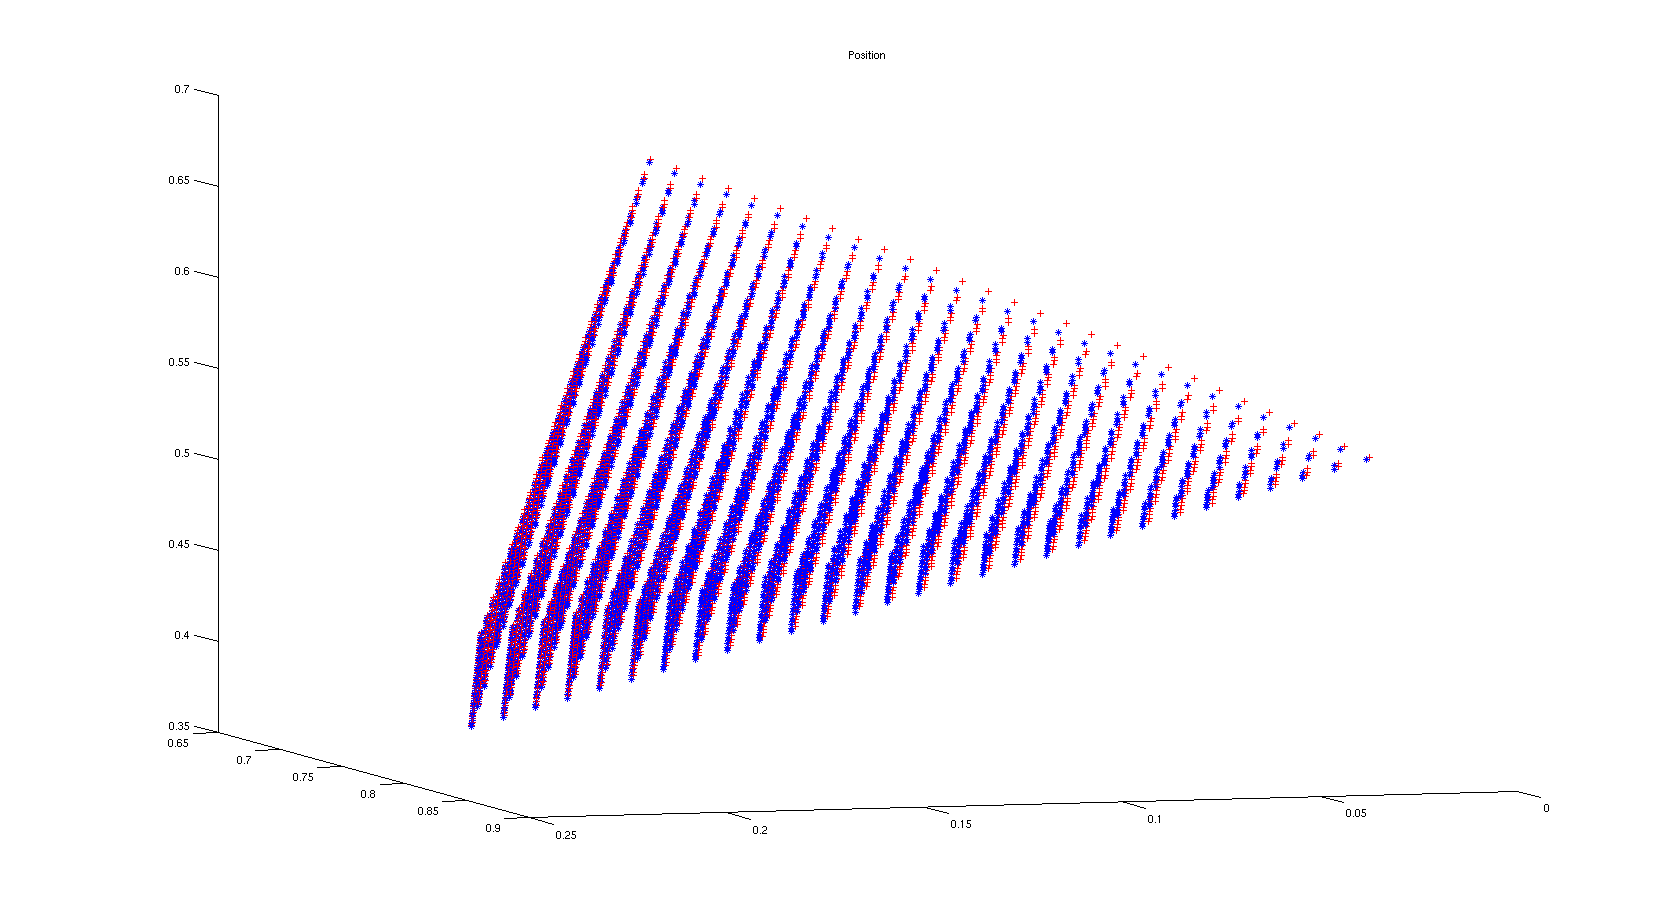
\includegraphics[width=0.7\textwidth]{pics/tetInnerNodes} 
\caption{All interior nodes of one macro tetrahedron at refinement level 5.
Blue points are for constant and the red for projected coordinates.}
\label{fig:tet0Nodes}
\end{figure}   

Since we are only interest in stencils within macro tetrahedra, and not in macro faces,
edges and vertices, we will now change our point of view and refer to these interior points
as \emph{tetrahedron}, where the four outermost nodes form its \emph{corners}. 
And all nodes lying on a straight between two corner nodes are denoted as \emph{edge}.


Now we will have a closer look on the stencils for this tetrahedron. As it is difficult 
to visualize 15-dimensional values in the 3-dimensional space, the tetrahedron is
cut into slices $S_k$, $k = 1,...,n_E$, corresponding to planes formed by the nodes
with constant coordinates.
$n_E$ is the number of nodes along one edge, with
\begin{equation}
n_E = 2^l-3.
\end{equation}
And in slice $S_k$, there are
\begin{equation}
n_{S_k} = k(k+1)/2
\end{equation}
points.

We reduce the 3-dimensional space to 2D by the simple projection $(x,y,z) \mapsto (x,y)$.
Note, that for each slice $S_k$ this is an bijective mapping, as 
$z = z(x,y)\enspace\forall(x,y,z)\in S_k$ and as long as $S_k$ is not orthogonal to the
z-axis. Now, the stencils can be visualized by using
the mapped spatial coordinates and plotting $\si$ in z-direction. 
In Fig.~\ref{fig:stencilCCvsVC} some $\si$ are illustrated for $S_{n_E}$. This is a
random selection as all of the $\si$ exhibit a similar shape. This also holds for other
$S_k$.
Naturally, as we consider here only constant coefficients, the particular stencil values 
for constant coordinates are equal for all nodes of the tetrahedron. Whereas for projected
coordinates we can observe some displacement. However, these displacements seem to
be a smooth function with some curvature in it. This motivates the assumption, that each
$\si$ can be fitted by a polynomial model. Due to the curvature, a linear fit is likely 
to be inaccurate, but quadratic polynomial may due it. So in the following we will 
investigate this approach.
Going to higher degrees may give additional accuracy, but will also increase the 
implantation complexity and computational costs. Therefore we will stick to the 
quadratic approach.


\begin{figure}\centering
\begin{tabular}{@{}cc@{}}
\includegraphics[width=0.475\textwidth]%
{pics/stencilMC_nE} &
\includegraphics[width=0.475\textwidth]%
{pics/stencilBC_nE} \\
(a) MC & (b) BC  \\

\includegraphics[width=0.475\textwidth]%
{pics/stencilMN_nE} &
\includegraphics[width=0.475\textwidth]%
{pics/stencilMSE_nE} \\
(c) MN & (d) MSE  \\

\includegraphics[width=0.475\textwidth]%
{pics/stencilMW_nE} &
\includegraphics[width=0.475\textwidth]%
{pics/stencilTSE_nE} \\
 (e) MW  & (f) TSE  \\
 
\includegraphics[width=0.475\textwidth]%
{pics/stencilBNW_nE} &
\includegraphics[width=0.475\textwidth]%
{pics/stencilTS_nE} \\
 (g) BNW  & (h) TS  
\end{tabular}
\caption{Eight out 15 stencil values for constant (blue) and projected
coordinates (red) for slice $S_{n_E}$.
\label{fig:stencilCCvsVC}}
\end{figure}  

\end{section}

%%%%%%%%%%%%%%%%%%%%%%%%%%%%%%%%%%%%%%%%%%%%%%%%%%%%%%%%%%%%%%%%%%%%%%%%%%%%%%%%%%%%%%%
%               Stencils for constant and projected coordinates                       %
%%%%%%%%%%%%%%%%%%%%%%%%%%%%%%%%%%%%%%%%%%%%%%%%%%%%%%%%%%%%%%%%%%%%%%%%%%%%%%%%%%%%%%%

\begin{section}{Interpolation of stencils}
For quadratic interpolation within on tetrahedron we choose the ansatz function
\begin{equation}
\label{eq:quadraticPolynomial}
a_{200}x^2 + a_{020}y^2 + a_{002}z^2 + a_{110}xy + a_{101}xz + a_{011}yz + 
a_{100}x + a_{010}y + a_{001}z + a_{000}
\end{equation}
Therefore we have to compute 10 coefficients $a_{(\cdot\cdot\cdot)}$, that is we
have to choose 10 sample points. Naturally, we choose the four corner nodes plus the six
edge midnodes, see Fig.~\ref{fig:samplePoints}

\begin{figure}\centering
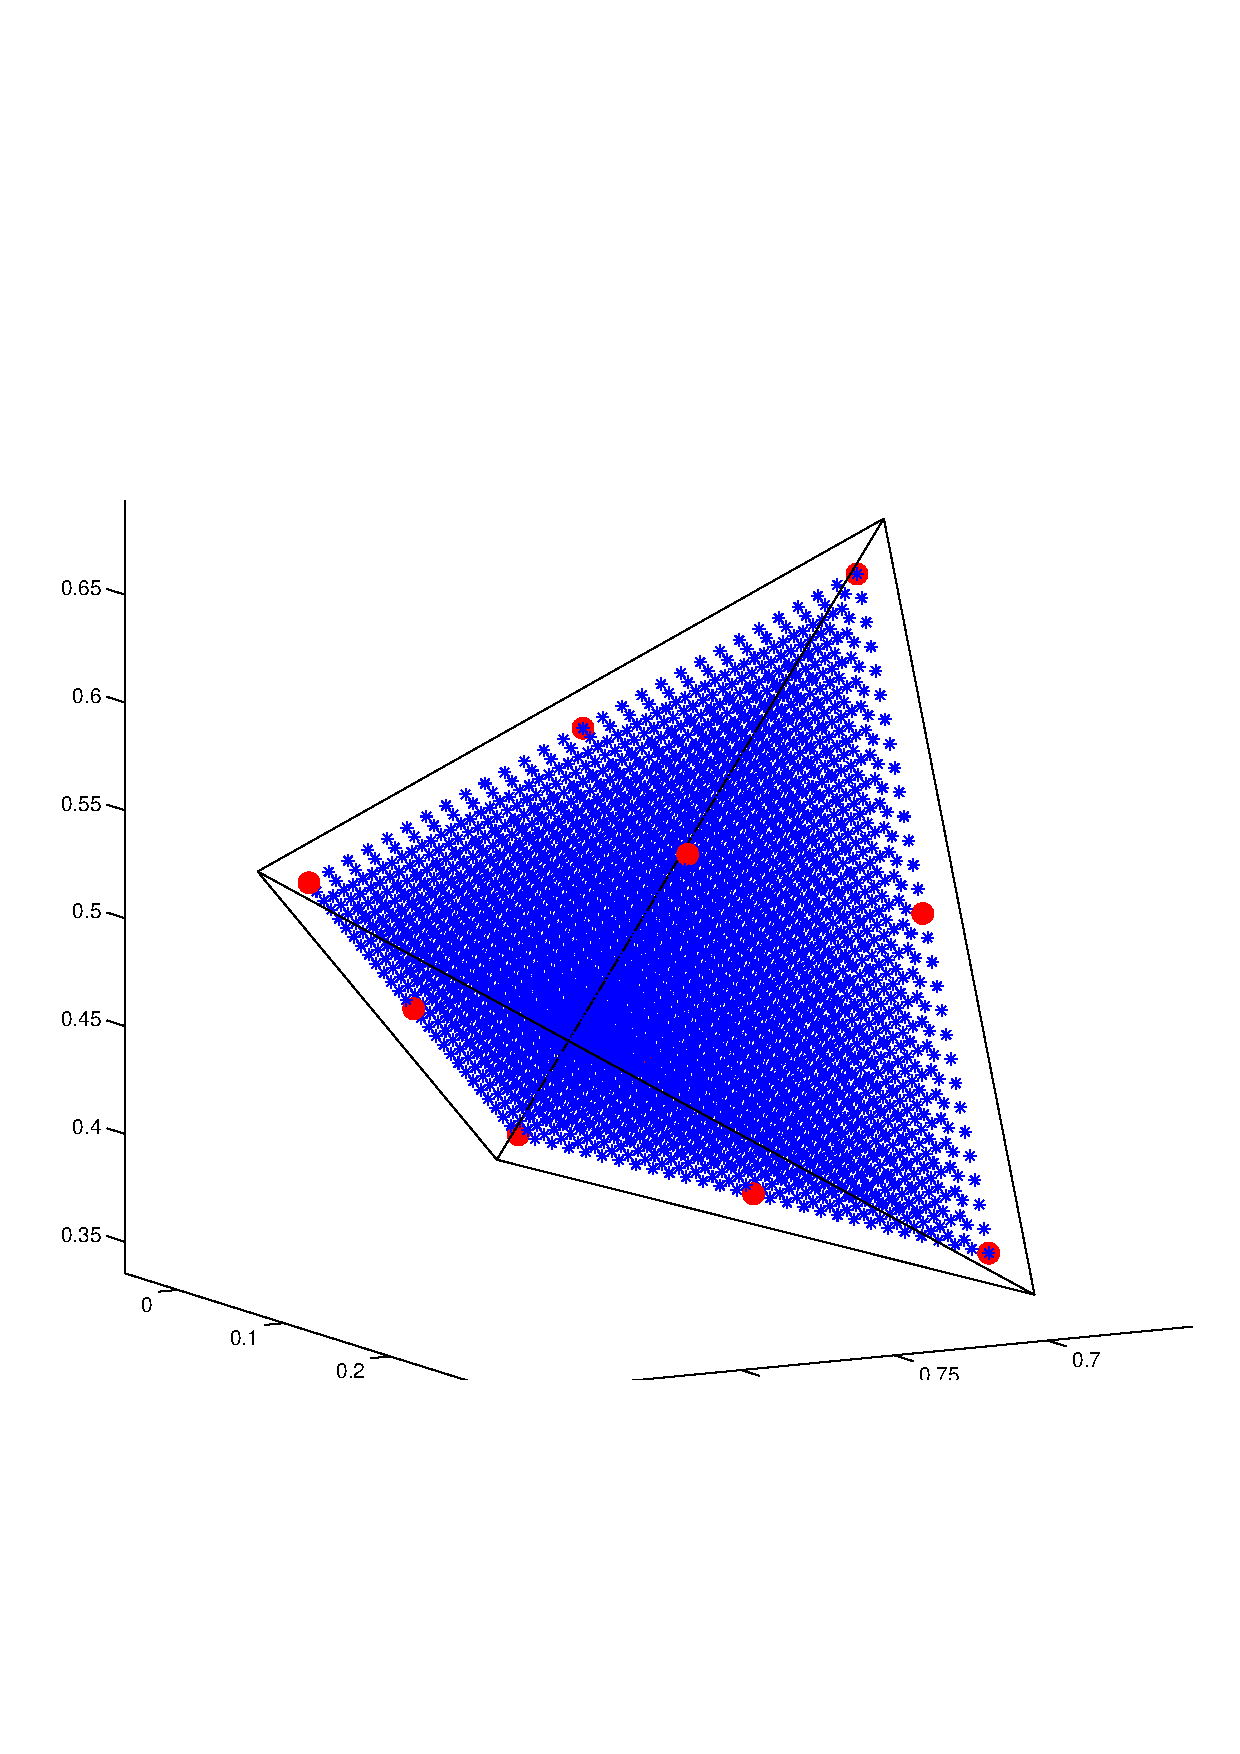
\includegraphics[width=0.7\textwidth]{pics/tetSamplePoints} 
\caption{Ten sample points (red) for quadratic interpolation of stencil values for 
all interior nodes (blue) within on macro tetrahedron (black). For visualization,
the constant coordinates have been used, but for the interpolation the projected
will be utilized.}
\label{fig:samplePoints}
\end{figure}  


\begin{subsection}{HHG Implementation}
In HHG this approach is realized by defining two new kernels 
\emph{tet\_gs\_coordsInterpolate.cc}
and \emph{tet\_residual\_coordsInterpolate.cc} based on \emph{tet\_gs\_coords.cc} and 
\emph{tet\_gs\_coords.cc}. As the stencil setup for gs and residual is the same, 
the modifications are identic in both files.

First, all $\si$ are computed for the ten sample points like in the original kernel. 
Additionally the (projected) x,y,z coordinates are used to build the $10\times10$ 
matrix $A$, with 
$A_{j,:} = \left[x_j^2\quad y_j^2\quad z_j^2\quad x_jy_j\quad x_jz_j\quad y_jz_j\quad
x_j\quad y_j\quad z_j\quad 1\right]$, $j = 1,...,10$.
Furthermore, the ten sample stencils are stored in a $10\times15$ matrix B,
with $B_{j,i} = \left(\si\right)_j$, $i = 1,...,15$, $j=1,...,10$. 
As this approach is intended to work 
also for tensor valued operators, e.g. full tensor, this scheme is repeated for each
operator entry, i.e, we have $A[op]$ and $B[op]$.

Note, that for each stencil entry we need one interpolation polynomial, i.e. we
have to compute $15\cdot10$ coefficients $a_{(\cdot\cdot\cdot)}^i$. To get these
coefficients one has to solve the linear system $Ax_i = B_{:,i}$,
where $x_i$ represents the coefficient vector for stencil entry $i$.

To this end, we include LAPACK for solving this linear system 15 times. 
Note, that $A$ doesn't change, so in fact we have to do one LU-decomposition
and perform 15 forward and backward substitutions.

Technically $A[op]$ and $B[op]$ are linear arrays for passing them to LAPACK. 

Once the coefficients have been computed, the interpolation of the stencils for
all tetrahedra nodes is straight forward. For each node, get its (projected) coordinates
and insert them into \eqref{eq:quadraticPolynomial}. One evaluation
of this polynomial consists of 21 multiplications and 9 additions, so in total 
\textbf{30 FLOPS}. This has to be done 15 times. 

For consistency, the center stencil
entry MC is set to the negative sum of all other entries.
Note, that by the same argument as in theorem \ref{theorem:equivalence}
this is already guaranteed by construction.

In Fig.~\ref{fig:stencilInterpolateME} the interpolated stencil values are representative
given for the ME stencil entry. Here we used an input mesh resolution with 1920 elements.


\begin{figure}[H]\centering
\begin{tabular}{@{}cc@{}}
\includegraphics[width=0.475\textwidth]%
{pics/stencilME_slice1} &
\includegraphics[width=0.475\textwidth]%
{pics/stencilME_slice7} \\
(a) ME slice $S_{29}$ & (b) ME slice $S_{23}$  \\
\includegraphics[width=0.475\textwidth]%
{pics/stencilME_slice14} &
\includegraphics[width=0.475\textwidth]%
{pics/stencilME_slice21} \\
(c) ME slice $S_{16}$ & (d) ME slice $S_{9}$  \\
\end{tabular}
\caption{Interpolation (black circles) of stencil value ME (red for projected, and 
blue for constant coordinates) for different slices.
\label{fig:stencilInterpolateME}}
\end{figure}  


\end{subsection}


\end{section}



%%%%%%%%%%%%%%%%%%%%%%%%%%%%%%%%%%%%%%%%%%%%%%%%%%%%%%%%%%%%%%%%%%%%%%%%%%%%%%%%%%%%%%%
%               Interpolation of local element matrices                               %
%%%%%%%%%%%%%%%%%%%%%%%%%%%%%%%%%%%%%%%%%%%%%%%%%%%%%%%%%%%%%%%%%%%%%%%%%%%%%%%%%%%%%%%
\newpage
\begin{section}{Interpolation of local element matrices}
\label{sec:interpolationLocElementMat}

However, this approach cannot be utilized for variable coefficients, as non-smooth
changes in the coefficients are not resolved by the interpolation. But there is a 
workaround. Instead of interpolating the stencils, we can interpolate the local 
element matrices and build the stencil by evaluating the interpolation polynomial
instead of computing the element matrices. As there are 24 surrounding fine grid
tetrahedra for each interior point, and for each of these there are 4 element matrix
entries that contribute to the stencil, we need in total 96 polynomials.

In following we will show, that for coefficients $c\equiv const$ (w.l.o.g. $const = 1$),
both interpolation approaches are equivalent.
Let $F_S : \RR^3 \rightarrow \RR^{15}$ be the representation of the 15pt stencil
for point $(x,y,z)$. Then the interpolation of the particular stencil entries reads
as
\begin{equation}
\label{eq:interpolationStencil}
F_S(x,y,z) = 
\begin{pmatrix}
f^1(x,y,z) \\
\vdots \\
f^{15}(x,y,z)
\end{pmatrix}
\approx
\begin{pmatrix}
p^f_1(x,y,z) \\
\vdots \\
p^f_{15}(x,y,z)
\end{pmatrix}
=: P^f(x,y,z)
\end{equation}
Where $p^f_i$ are quadratic polynomials.
On the other hand, $f^i$ is a sum over local element element matrix entries 
$e_j^i$ depending on $i$ ($i = 1,...,15$). 
Therefore, the interpolation of the local element matrices reads as

\begin{equation}
\label{eq:interpolationLocStiffness}
F_S(x,y,z) = 
\begin{pmatrix}
\sum_{j=1}^{n_1}e_j^1(x,y,z) \\
\vdots \\
\sum_{j=1}^{n_{15}}e_j^{15}(x,y,z) 
\end{pmatrix}
\approx
\begin{pmatrix}
\sum_{j=1}^{n_1}p_{1,j}^e(x,y,z)  \\
\vdots \\
\sum_{j=1}^{n_{15}}p_{15,j}^e(x,y,z) 
\end{pmatrix}
=: P^e(x,y,z)
\end{equation}
with quadratic polynomials $p^e_{i,j}$.

\begin{theorem}
\label{theorem:equivalence}
Both approaches are equivalent, i.e. $P^f = P^s$.
\end{theorem}
\begin{proof}
Throughout this proof it holds $i = 1,...,15$.
As $p^f_i$ and $p^e_{i,j}$ are quadratic polynomials, there exists 
a functional $\P_i : \RR^{10} \rightarrow \Pi^2$ which maps a
10-dimensional sample tuple linearly (and uniquely) 
onto a quadratic polynomial.

Let $f^i(x_k,y_k,z_k) =:f_k^i$ be the sample points
for $p^f_i$ and $e^i_j(x_k,y_k,z_k) =:e_{j,k}^i$ for $p^e_{i,j}$
with $k = 1,...,10$.
Then, it is
\begin{equation*}
\P_i(f^i_1,...,f^i_{10}) = p_i^f \in \Pi^2
\end{equation*}
and
\begin{equation*}
\P_i(e^i_{j,1},...,e^i_{j,10}) = p_{i,j}^e \in \Pi^2.
\end{equation*}
Then it holds for each $i= 1,...,15$
\begin{align*}
\begin{split}
P^e_i(x,y,z) &= \sum_{j=1}^{n_i} p^e_{i,j} 
 = \sum_{j=1}^{n_i}\left[\P_i\left(e^i_{j,1},...,e^i_{j,10}\right)(x,y,z)\right] \\
 &\stackrel{(1)}{=} \left[\sum_{j=1}^{n_i}\P_i\left(e^i_{j,1},...,e^i_{j,10}\right)\right](x,y,z) \\
 &\stackrel{(2)}{=} \P_i\left(\sum_{j=1}^{n_i}\left(e^i_{j,1},...,e^i_{j,10}\right)\right)(x,y,z) \\
 &\stackrel{(3)}{=} \P_i\left(\sum_{j=1}^{n_i}e^i_{j,1},...,\sum_{j=1}^{n_i}e^i_{j,10}\right)(x,y,z) \\
 &= \P_i\left(f^i_1,...,f^i_{10}\right)(x,y,z) \\
 &= p_i^f(x,y,z) = P_i^f(x,y,z).
\end{split}
\end{align*}
(1) addition of $\Pi^2$ elements\\
(2) $\P_i$ is linear \\
(3) basic vector addition\\
And therefore, $P^f = P^s$.
\end{proof}

\end{section}





%%%%%%%%%%%%%%%%%%%%%%%%%%%%%%%%%%%%%%%%%%%%%%%%%%%%%%%%%%%%%%%%%%%%%%%%%%%%%%%%%%%%%%%
%               Operation counts                                                     %
%%%%%%%%%%%%%%%%%%%%%%%%%%%%%%%%%%%%%%%%%%%%%%%%%%%%%%%%%%%%%%%%%%%%%%%%%%%%%%%%%%%%%%%

\clearpage

\begin{section}{Operation counts}
\label{sec:operationCounts}
%
Number of operations for a single lattice update for a scalar operator:\\
%
\begin{tabular}{c|c|c|c|c|c}
 \textbf{Coords} & \textbf{Coeffs} & \textbf{Interp} & \textbf{elem-mat} & \textbf{Adds/Mults} & \textbf{Divs} \\
 \hline
 constant  & constant & no  & 0  & \textbf{29}$^1$                                    & 0     \\
 constant  & variable & no  & 0  & 16$^2$ + 181$^3$ + 29$^1$ = \textbf{226}           & 1$^4$ \\
 projected & constant & no  & 24 & 181$^3$ + 29$^1$ = \textbf{210}                    & 1$^4$ \\
 projected & variable & no  & 24 & 32$^2$ + 181$^3$ + 29$^1$ = \textbf{242}           & 1$^4$ \\
 projected & constant & yes & 0  & 6$^5$ + 285$^6$ + 29$^1$ = \textbf{320}            & 1$^4$ \\
 projected & variable & yes & 0  & 6$^5$ + 32$^2$ + 1728$^6$ + 29$^1$ = \textbf{1795} & 1$^4$ \\
\end{tabular}\\
%
1: Stencil application\\
2: Averaging of viscosities\\
3: Coefficients times local element matrices\\
4: Calculation of central stencil entry\\
5: Calculating the coordinate-part of the interpolation polynomial ($x^2$, $x \cdot y$, etc)\\
6: Interpolation\\

Fenics reports 53 operations for the calculation of a Laplacian element matrix, so disregarding the divisions we would get:\\
%
\begin{tabular}{c|c|c|c|c|c|c}
 \textbf{Coords} & \textbf{Coeffs} & \textbf{Interp} & \textbf{Adds/Mults} & \textbf{maxlvl=4} & \textbf{maxlvl=5} & \textbf{maxlvl=6} \\
 \hline
 constant  & constant & no  & 29   & 0.046 & 0.16 & 0.77 \\
 constant  & variable & no  & 226  & 0.16  & 0.69 & 4.6  \\
 projected & constant & no  & 1482 & 0.96  & 8.1  & 71   \\
 projected & variable & no  & 1514 & 0.98  & 8.3  & 72   \\
 projected & constant & yes & 320  & 0.29  & 0.95 & 6.0  \\
 projected & variable & yes & 1795 & 0.76  & 5.5  & 46   \\
\end{tabular}\\
Also shown are runtimes for a regularly refined icosahedron (ntan=2, nrad=2) for different fine grid resolutions (serial, on borgcube, in seconds).

Calculating the local element matrices involves function calls, which could be slow.\\

\end{section}





%%%%%%%%%%%%%%%%%%%%%%%%%%%%%%%%%%%%%%%%%%%%%%%%%%%%%%%%%%%%%%%%%%%%%%%%%%%%%%%%%%%%%%%
%              Polynomial increment                                                   %
%%%%%%%%%%%%%%%%%%%%%%%%%%%%%%%%%%%%%%%%%%%%%%%%%%%%%%%%%%%%%%%%%%%%%%%%%%%%%%%%%%%%%%%

\clearpage

\begin{section}{Polynomial increment }
\label{sec:polynomialIncrement }
%
As the naiive polynomial evalution is rather expensive, we will
introduce a smarter way to do this.

Lets start with the Taylor expansion of a quadratic polynomial $p(x+h)$ (in 1D) 
at sample location $x$
\begin{equation}
p(x+h) = p(x) + p'(x)h + \frac{p''(x)}{2}h^2
\end{equation}
As it is quadratic, this representation is exact.
It is
\begin{equation}
p'(x) = 2ax+b,\qquad p''(x) = 2a
\end{equation}
Further, we introduce 
\begin{equation}
\delta p  := p'(x)h + \frac{p''(x)}{2}h^2 = (2ax+b)h + ah^2
\end{equation}
Now, lets do the same for $p((x+h)+h)$:
\begin{align}
\begin{split}
p(x+h+h) &= p(x+h) + p'(x+h)h + \frac{p''(x+h)}{2}h^2 \\
  &= p(x+h) + (2a(x+h)+b)h + ah^2 \\
  &= p(x+h) + \delta p + 2ah^2 \\
  &= p(x+h) + \delta p +\delta k
\end{split}
\end{align}
That is, we can evaluate the polynomial by simply
adding the increment $\delta p$ to the previous 
value and then updating $\delta p$ by $\delta k$ 
which is constant. This approach transfers straight
forward to 3D. Here we have

\begin{equation}
p(x,y,z) = a_{200}x^2 + a_{020}y^2 + a_{002}z^2 + a_{110}xy + a_{101}xz + a_{011}yz + 
a_{100}x + a_{010}y + a_{001}z + a_{000}
\end{equation}
and
\begin{align}
\begin{split}
p_x    &= 2a_{200}x+a_{110}y + a_{101}z + a_{100},\qquad p_{xx} = 2a_{200}\\
p_y    &= 2a_{020}y+a_{110}x + a_{011}z + a_{010},\qquad p_{yy} = 2a_{020}\\
p_z    &= 2a_{002}z+a_{101}x + a_{011}y + a_{001},\qquad p_{zz} = 2a_{002}
\end{split}
\end{align}

The algorithm is illustrated in Alg.~\ref{alg:polyincrement3D}


\begin{algorithm}[H]
 \KwData{$p(x,y,z)$ and its derivatives $p_x,p_{xx},p_y,p_{yy}, p_z,p_{zz}$ at location $(1,1,1)$\\
 $\delta kx = 2a_{200}h_x^2,\quad\delta ky = 2a_{020}h_y^2,\quad\delta kx = 2a_{002}h_z^2$\\
 $nX,nY,nZ$: number of sample points in $x,y,z$ direction}
 $\delta p_x = p_x h_x + \frac{p_{xx}}{2} h_x^2$\;
 $\delta p_y = p_y h_y + \frac{p_{yy}}{2} h_y^2$\;
 $\delta p_z = p_z h_z + \frac{p_{zz}}{2} h_z^2$\;
 \For{$K=1:nZ$}{
  \If{$K > 1$}{
   $p(K,1,1) = p(K-1,1,1)+\delta pz$\;
   $\delta pz = \delta pz + \delta kz$\;
   
   $\delta py = \delta py(K,1,1)$\;
   $\delta px = \delta px(K,1,1)$\;
   }
   
   
   \For{$J=1:nY$}{
      \If{$J > 1$}{
         $p(K,J,1) = p(K,J-1,1)+\delta py$\;
         $\delta py = \delta py + \delta ky$\;
   
         $\delta px = \delta px(K,J,1)$\;
      }
      
      
      \For{$I=2:nX$}{
         $p(K,J,I) = p(K,J,I-1)+\delta px$\;
         $\delta px = \delta px + \delta kx$\;
      }
    }
 }   
 \caption{Evaluation of 3D quadratic polynomial by increments}
 \label{alg:polyincrement3D}
\end{algorithm}










\end{section}





%%%%%%%%%%%%%%%%%%%%%%%%%%%%%%%%%%%%%%%%%%%%%%%%%%%%%%%%%%%%%%%%%%%%%%%%%%%%%%%%%%%%%%%
%               Spherepoisson test                                                    %
%%%%%%%%%%%%%%%%%%%%%%%%%%%%%%%%%%%%%%%%%%%%%%%%%%%%%%%%%%%%%%%%%%%%%%%%%%%%%%%%%%%%%%%
\begin{section}{Spherepoisson test}



For evaluation of these new approaches, let us begin with the spherepoisson driver, 
and an initial input grid with 
540 macro tetrahedra (i.e ntan=4, nrad=2). We run the test problem for several
maximal refinement levels (starting with 3 and going up to level 7) in parallel
with 32 processors. In Fig.~\ref{fig:spherepoissonRES_3}-\ref{fig:spherepoissonERR_3}
the residual, CPU time and discretisation error, respectively, are shown.
In Fig.~\ref{fig:spherepoissonRES_3} we can observe a very good match for
projected coordinates and the interpolation
approaches (as there is no red line visible).
And according to our theoretical statement, both interpolation approaches are
equivalent. But the difference gets obvious when we have a look at the CPU time,
cf. Fig.~\ref{fig:spherepoissonCPU_3}. The runtime for stencil interpolation
gets pretty close to the constant case, whereas for interpolated element matrices
there is only some moderate speed up compared to projected coordinates.
This behavior represents also the theoretical operation counts in section 
\ref{sec:operationCounts}.
For the discretisation error, we expect a reduction
of factor 4 for each refinement. This holds for the constant and for the projected
coordinates cases, as can be seen in Fig.~\ref{fig:spherepoissonERR_3}. But for
the interpolation this only holds for level 3,4 and 5, at level 6 and 7 it deteriorates.
This can be seen more clearly in Fig.~\ref{fig:spherepoissonERR_compare}.

For a better interpretation of these results, lets have a look at the stencil values itself.
Therefore, we compute for each sample point the norm of the stencil as $\|F_S\|_2$ 
(see section \ref{sec:interpolationLocElementMat}).
In Fig.~\ref{fig:stencilNormPoisson} (a) these norms are plotted for all macro tetrahedra.
As these are somewhat difficult to interpret, we additionally compute the mean value
of these norms (b). 

Assuming that all non-center stencil entries are approximately of the same order,
i.e. they have value $v$, then the L2 norm reads as
\begin{equation}
\|F_S\|_2 \approx \sqrt{\sum_{i=1}^{14}v^2 + \left(\sum_{i=1}^{14}-v\right)^2}
= \sqrt{210 v^2} \approx 15v
\end{equation}



\begin{figure}[H]\centering
\begin{tabular}{@{}cc@{}}
\includegraphics[width=0.475\textwidth]%
{pics/spherepoisson_resEuc_level4.eps} &
\includegraphics[width=0.475\textwidth]%
{pics/spherepoisson_resEuc_level5.eps} \\
(a) max. level 4 & (b) max. level 5  \\
\includegraphics[width=0.475\textwidth]%
{pics/spherepoisson_resEuc_level6.eps} &
\includegraphics[width=0.475\textwidth]%
{pics/spherepoisson_resEuc_level7.eps} \\
(c) max. level 6 & (d) max. level 7  
\end{tabular}
\caption{Residual in L2-Norm for spherepoisson driver
for constant (blue) and projected (red) coordinates,
for interpolated (green) stencils and for interpolated
element matrices (magenta)for different
levels of maximal refinement.
\label{fig:spherepoissonRES_3}}
\end{figure}  


\begin{figure}[H]\centering
\begin{tabular}{@{}cc@{}}
\includegraphics[width=0.475\textwidth]%
{pics/spherepoisson_cpuTime_level4.eps} &
\includegraphics[width=0.475\textwidth]%
{pics/spherepoisson_cpuTime_level5.eps} \\
(a) max. level 4 & (b) max. level 5  \\
\includegraphics[width=0.475\textwidth]%
{pics/spherepoisson_cpuTime_level6.eps} &
\includegraphics[width=0.475\textwidth]%
{pics/spherepoisson_cpuTime_level7.eps} \\
(c) max. level 6 & (d) max. level 7  
\end{tabular}
\caption{CPU time for spherepoisson driver
for constant (blue) and projected (red) coordinates,
for interpolated (green) stencils and for interpolated
element matrices (magenta) for parallel runs with
32 processors.
\label{fig:spherepoissonCPU_3}}
\end{figure}  


\begin{figure}[H]\centering
\begin{tabular}{@{}cc@{}}
\includegraphics[width=0.475\textwidth]%
{pics/spherepoisson_errorEuc_level4.eps} &
\includegraphics[width=0.475\textwidth]%
{pics/spherepoisson_errorEuc_level5.eps} \\
(a) max. level 4 & (b) max. level 5  \\
\includegraphics[width=0.475\textwidth]%
{pics/spherepoisson_errorEuc_level6.eps} &
\includegraphics[width=0.475\textwidth]%
{pics/spherepoisson_errorEuc_level7.eps} \\
(c) max. level 6 & (d) max. level 7  
\end{tabular}
\caption{Discretisation error in L2-Norm for 
spherepoisson driver
\label{fig:spherepoissonERR_3}}
\end{figure}  





\begin{figure}[H]\centering
\begin{tabular}{@{}cc@{}}
\includegraphics[width=0.4\textwidth]%
{pics/spherepoisson_errorEuc_ProjCoords.eps} &
\includegraphics[width=0.4\textwidth]%
{pics/spherepoisson_errorEuc_InterpolationStencil.eps} 
\end{tabular}
\caption{Discretisation error for projected coordinates (left)
and interpolated stencils (right).
\label{fig:spherepoissonERR_compare}}
\end{figure}  


\begin{figure}[H]\centering
\begin{tabular}{@{}cc@{}}
\includegraphics[width=0.475\textwidth]%
{pics/stencilNormPoisson_ntan4.eps} &
\includegraphics[width=0.475\textwidth]%
{pics/meanStencilValuePoisson_ntan4.eps} 
\end{tabular}
\caption{Stencil norms of 10 sample points for all 
macro tetrahedra
(incl. mean value as horizontal line)
(left)
and their mean values (right) on different levels.
\label{fig:spherepoissonERR_compare}}
\end{figure}  


\begin{remark}
For all element matrix interpolation runs, we had to use 
\emph{useOpsForVarCoeffs=false}, manually set the coefficients to
1 in the \emph{tet\_gs\_coeff\_coordsInterpolate.cc} and \\
\emph{tet\_residual\_coeff\_coordsInterpolate.cc} kernels and finally substitute
tet\_gs\_coordsInterpolate.cc/ tet\_residual\_coordsInterpolate by these two
kernels.
This was necessary (as we suppose) due to bug in the faces kernel where
the coefficients are not set correctly. Otherwise the results deteriorate.
\end{remark}





% compare different approaches

% \begin{figure}[H]\centering
% \begin{tabular}{@{}cc@{}}
% \includegraphics[width=0.475\textwidth]%
% {pics/spherepoisson_resEuc_2_level3.eps} &
% \includegraphics[width=0.475\textwidth]%
% {pics/spherepoisson_resEuc_2_level4.eps} \\
% (a) max. level 3 & (b) max. level 4  \\
% \includegraphics[width=0.475\textwidth]%
% {pics/spherepoisson_resEuc_2_level5.eps} &
% \includegraphics[width=0.475\textwidth]%
% {pics/spherepoisson_resEuc_2_level6.eps} \\
% (c) max. level 5 & (d) max. level 6  
% \end{tabular}
% \end{figure}  
% 
% 
% 
% \begin{figure}[H]\centering
% \begin{tabular}{@{}cc@{}}
% \includegraphics[width=0.475\textwidth]%
% {pics/spherepoisson_errorEuc_2_level3.eps} &
% \includegraphics[width=0.475\textwidth]%
% {pics/spherepoisson_errorEuc_2_level4.eps} \\
% (a) max. level 3 & (b) max. level 4  \\
% \includegraphics[width=0.475\textwidth]%
% {pics/spherepoisson_errorEuc_2_level5.eps} &
% \includegraphics[width=0.475\textwidth]%
% {pics/spherepoisson_errorEuc_2_level6.eps} \\
% (c) max. level 5 & (d) max. level 6  
% \end{tabular}
% \end{figure}  



\begin{figure}[H]\centering
\begin{tabular}{@{}cc@{}}
\includegraphics[width=0.49\textwidth]%
{pics/spherepoisson_resEuc_2_level3.eps} &
\includegraphics[width=0.49\textwidth]%
{pics/spherepoisson_errorEuc_2_level3.eps} \\
\includegraphics[width=0.49\textwidth]%
{pics/spherepoisson_resEuc_2_level4.eps} &
\includegraphics[width=0.49\textwidth]%
{pics/spherepoisson_errorEuc_2_level4.eps} \\
\includegraphics[width=0.49\textwidth]%
{pics/spherepoisson_resEuc_2_level5.eps} &
\includegraphics[width=0.49\textwidth]%
{pics/spherepoisson_errorEuc_2_level5.eps} \\
\includegraphics[width=0.49\textwidth]%
{pics/spherepoisson_resEuc_2_level6.eps} &
\includegraphics[width=0.49\textwidth]%
{pics/spherepoisson_errorEuc_2_level6.eps} 
\end{tabular}
\caption{Ntan=4, i.e. 540 macro tetrahedra}
\end{figure}  


\begin{figure}[H]\centering
\begin{tabular}{@{}cc@{}}
\includegraphics[width=0.49\textwidth]%
{pics/spherepoisson_resEuc_ntan2_level3.eps} &
\includegraphics[width=0.49\textwidth]%
{pics/spherepoisson_errorEuc_ntan2_level3.eps} \\
\includegraphics[width=0.49\textwidth]%
{pics/spherepoisson_resEuc_ntan2_level4.eps} &
\includegraphics[width=0.49\textwidth]%
{pics/spherepoisson_errorEuc_ntan2_level4.eps} \\
\includegraphics[width=0.49\textwidth]%
{pics/spherepoisson_resEuc_ntan2_level5.eps} &
\includegraphics[width=0.49\textwidth]%
{pics/spherepoisson_errorEuc_ntan2_level5.eps} \\
\includegraphics[width=0.49\textwidth]%
{pics/spherepoisson_resEuc_ntan2_level6.eps} &
\includegraphics[width=0.49\textwidth]%
{pics/spherepoisson_errorEuc_ntan2_level6.eps} 
\end{tabular}
\caption{Ntan=2, i.e. 60 macro tetrahedra}
\end{figure}  


\begin{figure}[H]\centering
\begin{tabular}{@{}cc@{}}
\includegraphics[width=0.49\textwidth]%
{pics/spherepoisson_cpuTime_ntan2_level5.eps} &
\includegraphics[width=0.49\textwidth]%
{pics/spherepoisson_cpuTime_ntan2_level6.eps} \\
% \includegraphics[width=0.49\textwidth]%
% {pics/spherepoisson_cpuTime_ntan2_level4.eps} &
% \includegraphics[width=0.49\textwidth]%
% {pics/spherepoisson_cpuTime_ntan2_level4.eps} \\
% \includegraphics[width=0.49\textwidth]%
% {pics/spherepoisson_cpuTime_ntan2_level5.eps} &
% \includegraphics[width=0.49\textwidth]%
% {pics/spherepoisson_cpuTime_ntan2_level5.eps} \\
% \includegraphics[width=0.49\textwidth]%
% {pics/spherepoisson_cpuTime_ntan2_level6.eps} &
% \includegraphics[width=0.49\textwidth]%
% {pics/spherepoisson_cpuTime_ntan2_level6.eps} 
% \caption{Ntan=2, i.e. 60 macro tetrahedra}
\end{tabular}
\caption{Ntan=2, i.e. 60 macro tetrahedra}
\end{figure}  


%-----------------------------------------















\end{section}








%%%%%%%%%%%%%%%%%%%%%%%%%%%%%%%%%%%%%%%%%%%%%%%%%%%%%%%%%%%%%%%%%%%%%%%%%%%%%%%%%%%%%%%
%               Spherestokes test                                                    %
%%%%%%%%%%%%%%%%%%%%%%%%%%%%%%%%%%%%%%%%%%%%%%%%%%%%%%%%%%%%%%%%%%%%%%%%%%%%%%%%%%%%%%%
\begin{section}{Spherestokes test}


For the Stokes problem, we observe, in contrast to the Poisson case,
a very good match between the projected coordinates and interpolation,
cf. Fig.~\ref{fig:spherestokesRES_3} - \ref{fig:spherestokesERR_3}

One possible explanation:
As we do Schur complement CG, the inverse of $A$ is only 
approximated by a few V-cycles. So we do not enter the 
critical zone where the discretisation error
gets stagnant. Furthermore the outer CG iteration may 
smear out/eliminate the error introduced by interpolation.

Note, that this only holds, if only the $A$ part is approximated by
interpolation. For the $B$ part we still have to explicitly compute the
stencils. But Fig.~\ref{fig:spherestokesCPU_3} shows that this has only
minor impact on the runtime.

So maybe we do not need to be so accurate for the $A$ part. What happens
if we use linear interpolation, which reduces the amount of work by
factor of 3? See 
Fig.~\ref{fig:spherestokesLinearRES_3} - \ref{fig:spherestokesLinearERR_3}.


\begin{figure}[H]\centering
\begin{tabular}{@{}cc@{}}
\includegraphics[width=0.475\textwidth]%
{pics/spherestokes_resEuc_intP_level3.eps} &
\includegraphics[width=0.475\textwidth]%
{pics/spherestokes_resEuc_intP_level4.eps} \\
(a) max. level 3 & (b) max. level 4  \\
\includegraphics[width=0.475\textwidth]%
{pics/spherestokes_resEuc_intP_level5.eps} &
\includegraphics[width=0.475\textwidth]%
{pics/spherestokes_resEuc_intP_level6.eps} \\
(c) max. level 5 & (d) max. level 6  
\end{tabular}
\caption{Residual in L2-Norm for spherestokes driver
for constant (blue) and projected (red) coordinates,
for interpolated (green/cyan) stencils and for interpolated
element matrices (magenta/black). For green and magenta
curve, only the $A$ part of the Stokes system is interpolated,
whereas for cyan and black also the $B$ part is interpolated.
\label{fig:spherestokesRES_3}}
\end{figure}  


\begin{figure}[H]\centering
\begin{tabular}{@{}cc@{}}
\includegraphics[width=0.475\textwidth]%
{pics/spherestokes_cpuTime_intP_level3.eps} &
\includegraphics[width=0.475\textwidth]%
{pics/spherestokes_cpuTime_intP_level4.eps} \\
(a) max. level 3 & (b) max. level 4  \\
\includegraphics[width=0.475\textwidth]%
{pics/spherestokes_cpuTime_intP_level5.eps} &
\includegraphics[width=0.475\textwidth]%
{pics/spherestokes_cpuTime_intP_level6.eps} \\
(c) max. level 5 & (d) max. level 6  
\end{tabular}
\caption{CPU time for spherestokes driver
for constant (blue) and projected (red) coordinates,
for interpolated (green/cyan) stencils and for interpolated
element matrices (magenta/black) for parallel runs with
32 processors.
For green and magenta
curve, only the $A$ part of the Stokes system is interpolated,
whereas for cyan and black also the $B$ part is interpolated.
\label{fig:spherestokesCPU_3}}
\end{figure}  


\begin{figure}[H]\centering
\begin{tabular}{@{}cc@{}}
\includegraphics[width=0.475\textwidth]%
{pics/spherestokes_errorEuc_intP_level3.eps} &
\includegraphics[width=0.475\textwidth]%
{pics/spherestokes_errorEuc_intP_level4.eps} \\
(a) max. level 3 & (b) max. level 4  \\
\includegraphics[width=0.475\textwidth]%
{pics/spherestokes_errorEuc_intP_level5.eps} &
\includegraphics[width=0.475\textwidth]%
{pics/spherestokes_errorEuc_intP_level6.eps} \\
(c) max. level 5 & (d) max. level 6  
\end{tabular}
\caption{Discretisation error in L2-Norm for 
spherestokes driver.
For green and magenta
curve, only the $A$ part of the Stokes system is interpolated,
whereas for cyan and black also the $B$ part is interpolated.
\label{fig:spherestokesERR_3}}
\end{figure}  



\begin{figure}[H]\centering
\begin{tabular}{@{}c}
\includegraphics[width=0.98\textwidth]%
{pics/meanStencilValueFullTensor_ntan4.eps} \\
\includegraphics[width=0.98\textwidth]%
{pics/meanStencilValueGradP_ntan4.eps} 
\end{tabular}
\caption{Mean stencil values for the full 
operator (top) and for grad operator (bottom)
\label{fig:spherestokesERR_compare}}
\end{figure}  














\begin{figure}[H]\centering
\begin{tabular}{@{}cc@{}}
\includegraphics[width=0.475\textwidth]%
{pics/spherestokes_resEuc_linear_level3.eps} &
\includegraphics[width=0.475\textwidth]%
{pics/spherestokes_resEuc_linear_level4.eps} \\
(a) max. level 3 & (b) max. level 4  \\
\includegraphics[width=0.475\textwidth]%
{pics/spherestokes_resEuc_linear_level5.eps} &
\includegraphics[width=0.475\textwidth]%
{pics/spherestokes_resEuc_linear_level6.eps} \\
(c) max. level 5 & (d) max. level 6  
\end{tabular}
\caption{Residual in L2-Norm for spherestokes driver
for constant (blue) and projected (red) coordinates,
for interpolated (green/cyan) stencils and for interpolated
element matrices (magenta/black). For green/magenta
curve, we do quadratic interpolation,
and for cyan/black linear interpolation.
\label{fig:spherestokesLinearRES_3}}
\end{figure}  


\begin{figure}[H]\centering
\begin{tabular}{@{}cc@{}}
\includegraphics[width=0.475\textwidth]%
{pics/spherestokes_cpuTime_linear_level3.eps} &
\includegraphics[width=0.475\textwidth]%
{pics/spherestokes_cpuTime_linear_level4.eps} \\
(a) max. level 3 & (b) max. level 4  \\
\includegraphics[width=0.475\textwidth]%
{pics/spherestokes_cpuTime_linear_level5.eps} &
\includegraphics[width=0.475\textwidth]%
{pics/spherestokes_cpuTime_linear_level6.eps} \\
(c) max. level 5 & (d) max. level 6  
\end{tabular}
\caption{CPU time for spherestokes driver
for constant (blue) and projected (red) coordinates,
for interpolated (green/cyan) stencils and for interpolated
element matrices (magenta/black) for parallel runs with
32 processors.
For green/magenta
curve, we do quadratic interpolation,
and for cyan/black linear interpolation.
\label{fig:spherestokesLinearCPU_3}}
\end{figure}  


\begin{figure}[H]\centering
\begin{tabular}{@{}cc@{}}
\includegraphics[width=0.475\textwidth]%
{pics/spherestokes_errorEuc_linear_level3.eps} &
\includegraphics[width=0.475\textwidth]%
{pics/spherestokes_errorEuc_linear_level4.eps} \\
(a) max. level 3 & (b) max. level 4  \\
\includegraphics[width=0.475\textwidth]%
{pics/spherestokes_errorEuc_linear_level5.eps} &
\includegraphics[width=0.475\textwidth]%
{pics/spherestokes_errorEuc_linear_level6.eps} \\
(c) max. level 5 & (d) max. level 6  
\end{tabular}
\caption{Discretisation error in L2-Norm for 
spherestokes driver.
For green/magenta
curve, we do quadratic interpolation,
and for cyan/black linear interpolation.
\label{fig:spherestokesLinearERR_3}}
\end{figure}  





\end{section}




% -----------------------------------------------------------------------------
\end{document}
% -----------------------------------------------------------------------------